\documentclass{article}

% Packages
\usepackage{graphicx} % Required for inserting images
\usepackage[utf8]{inputenc}
\usepackage[margin=1in]{geometry}
\usepackage{amsmath}
\usepackage{amssymb}
\usepackage{algorithm}
\usepackage{algorithmic}
\usepackage{listings}
\usepackage{xcolor}
\usepackage{hyperref}
\usepackage{caption}
\usepackage{subcaption}
\usepackage{booktabs}
\usepackage{float}
\usepackage{tikz}
\usetikzlibrary{shapes.geometric, arrows, positioning}

\title{Manga-pages to panel}
\author{Samip Shrestha}
\date{November 2025}

% Code styling
\lstset{
    language=Python,
    basicstyle=\ttfamily\small,
    keywordstyle=\color{blue},
    commentstyle=\color{green!60!black},
    stringstyle=\color{red},
    showstringspaces=false,
    breaklines=true,
    frame=single,
    numbers=left,
    numberstyle=\tiny\color{gray}
}

\begin{document}

\maketitle

\begin{abstract}
This document describes a system for automatically detecting comic/manga panels from page images. The approach uses computer vision techniques to find panel borders by analyzing dark content regions and their edges. It uses edge-based detection with gap tolerance to handle different comic layouts, and includes fallback logic when detection quality is low.
\end{abstract}

\tableofcontents
\newpage

\section{Introduction}

Comic panel segmentation is the process of automatically identifying and extracting individual panels from a comic or manga page. This is useful for creating audio narrations, videos, or making comics more accessible.

\subsection{Challenges}
Detecting panels is tricky because:
\begin{itemize}
    \item Panels have different shapes and sizes
    \item Gutters (space between panels) vary in width
    \item Some panels overlap or nest inside others
    \item Text and artwork can make borders unclear
    \item Comics read left-to-right, manga reads right-to-left
\end{itemize}

\subsection{Approach}
This system uses an edge-based method with:
\begin{itemize}
    \item Edge detection to find panel borders
    \item 20\% gap tolerance for incomplete borders
    \item Coverage checking to ensure quality results
    \item Reading order sorting for proper panel sequence
\end{itemize}

\section{How It Works}

The system processes a comic page through 6 steps. We'll use two real examples:
\begin{itemize}
    \item \textbf{Page p015}: Normal case with 6 panels detected (784×1145 pixels)
    \item \textbf{Page p008}: Low coverage case triggering full-page fallback (784×1145 pixels)
\end{itemize}

\begin{figure}[H]
\centering
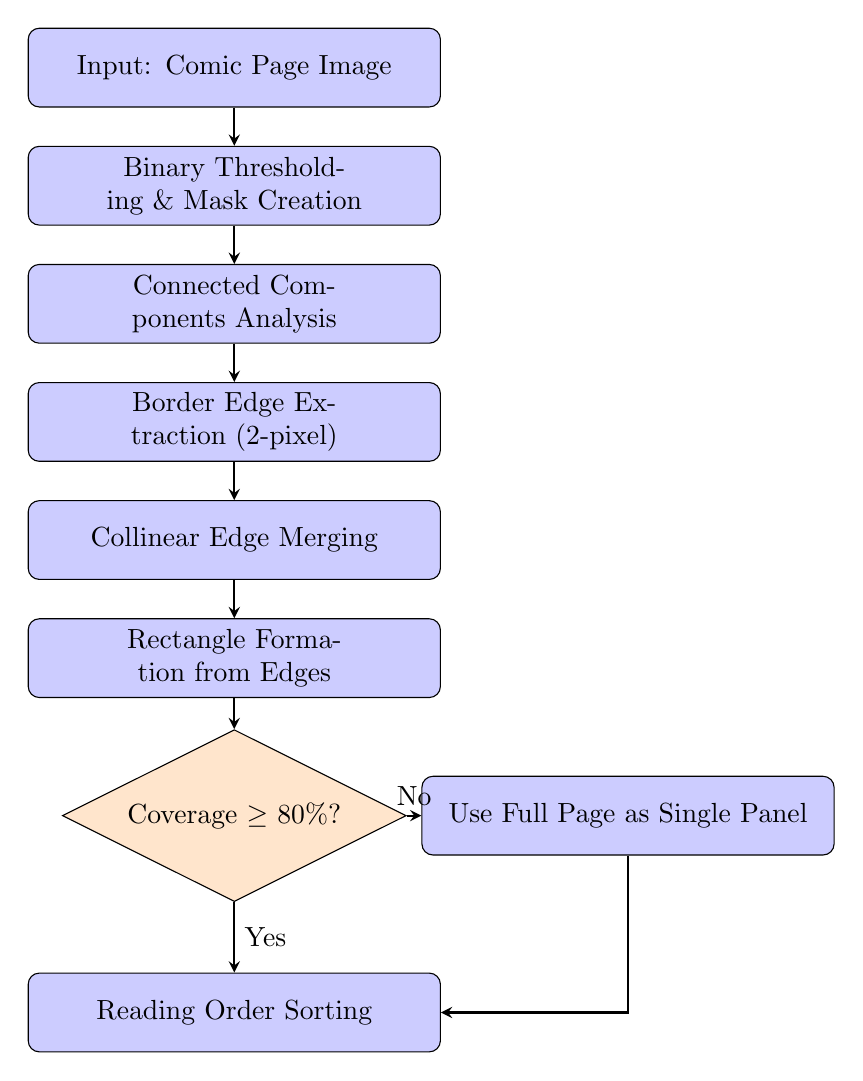
\begin{tikzpicture}[node distance=1.5cm, auto, 
    process/.style={rectangle, draw, fill=blue!20, text width=5cm, text centered, rounded corners, minimum height=1cm},
    decision/.style={diamond, draw, fill=orange!20, text width=3cm, text centered, aspect=2},
    arrow/.style={thick,->,>=stealth}]
    
    \node [process] (input) {Input: Comic Page Image};
    \node [process, below of=input] (threshold) {Binary Thresholding \& Mask Creation};
    \node [process, below of=threshold] (components) {Connected Components Analysis};
    \node [process, below of=components] (edges) {Border Edge Extraction (2-pixel)};
    \node [process, below of=edges] (merge) {Collinear Edge Merging};
    \node [process, below of=merge] (rectangles) {Rectangle Formation from Edges};
    \node [decision, below of=rectangles, node distance=2cm] (coverage) {Coverage $\geq$ 80\%?};
    \node [process, below of=coverage, node distance=2.5cm] (sort) {Reading Order Sorting};
    \node [process, right of=coverage, node distance=5cm] (fullpage) {Use Full Page as Single Panel};
    
    \draw [arrow] (input) -- (threshold);
    \draw [arrow] (threshold) -- (components);
    \draw [arrow] (components) -- (edges);
    \draw [arrow] (edges) -- (merge);
    \draw [arrow] (merge) -- (rectangles);
    \draw [arrow] (rectangles) -- (coverage);
    \draw [arrow] (coverage) -- node[right] {Yes} (sort);
    \draw [arrow] (coverage) -- node[above] {No} (fullpage);
    \draw [arrow] (fullpage) |- (sort);
\end{tikzpicture}
\caption{Comic Panel Segmentation Pipeline}
\label{fig:pipeline}
\end{figure}

\subsection{Step 1: Create Binary Mask}

\textbf{What it does:} Converts the image to grayscale and creates a binary mask where dark pixels (artwork, text) become white, and light pixels (gutters) become black. Uses a threshold of 50 on a 0-255 scale.

\textbf{Why it's needed:} Comic panels are separated by white space (gutters). By turning the image into just black and white, we can easily distinguish between "content" (the dark artwork) and "empty space" (the light gutters between panels). This makes it much easier to find where panels begin and end.

\textbf{Mathematical formulation:}
Given a grayscale image $G(x,y)$ where pixel intensities range from 0 (black) to 255 (white), we apply inverse binary thresholding:
\[
M(x,y) = \begin{cases} 
255 & \text{if } G(x,y) < \theta \\
0 & \text{if } G(x,y) \geq \theta
\end{cases}
\]
where $\theta = 50$ is our threshold value. This creates mask $M(x,y)$ where content pixels (dark) are white (255) and gutter pixels (light) are black (0).

\begin{figure}[H]
\centering
\includegraphics[width=0.45\textwidth]{tests/output/Dandadan - c003 (web) - p015 [Unknown]/01_original.jpg}
\includegraphics[width=0.45\textwidth]{tests/output/Dandadan - c003 (web) - p015 [Unknown]/04_border_edges.jpg}
\caption{Left: Original page. Right: Detected border edges (red lines show panel boundaries)}
\end{figure}

\begin{lstlisting}
# Convert to grayscale
gray = cv2.cvtColor(img, cv2.COLOR_BGR2GRAY)
height, width = gray.shape

# Create binary mask (dark areas become white)
_, black_mask = cv2.threshold(
    gray, 
    self.black_threshold,  # theta = 50
    255, 
    cv2.THRESH_BINARY_INV
)
\end{lstlisting}

\subsection{Step 2: Find Connected Components}

\textbf{What it does:} Identifies all continuous dark regions (content areas) in the mask using connected component analysis. Each region represents artwork, text, or other panel content.

\textbf{Why it's needed:} This is the \textit{critical foundation} that enables the entire edge-based detection approach. Without connected components analysis, edge detection would capture edges of everything in the image - character outlines, speech bubble borders, background details, and panel boundaries all mixed together, creating thousands of unusable false positives.

By first segmenting the image into 2,500+ individual content blobs, we can then extract edges \textit{per blob}. When we find that many different blobs share the same edge position (e.g., 20 different content regions all end at $x=300$), that common edge indicates a panel boundary rather than just content details. This per-blob analysis transforms noisy whole-image edges into clean panel boundaries.

\textbf{Mathematical formulation:}
We use 8-connectivity to label connected components. Two pixels $p_1(x_1,y_1)$ and $p_2(x_2,y_2)$ are 8-connected if:
\[
\max(|x_1-x_2|, |y_1-y_2|) = 1 \text{ and } M(x_1,y_1) = M(x_2,y_2) = 255
\]
This partitions the mask into $N$ disjoint regions $\{R_1, R_2, \ldots, R_N\}$ where each $R_i$ represents a connected content blob.

\begin{figure}[H]
\centering
\includegraphics[width=0.6\textwidth]{tests/output/Dandadan - c003 (web) - p015 [Unknown]/03_connected_components.jpg}
\caption{Connected components colored uniquely (6,050 components found)}
\end{figure}

\textbf{Example outputs:}
\begin{itemize}
    \item Page p015: 6,050 content patches found
    \item Page p008: 5,459 content patches found (more complex artwork)
\end{itemize}

\subsection{Step 3: Extract Border Edges}

\textbf{What it does:} For each content region found in Step 2, extracts the edges by finding the topmost, bottommost, leftmost, and rightmost 2-pixel borders. Only edges that are long enough (15\% of width for horizontal, 10\% of height for vertical) and continuous enough (80\%) are kept.

\textbf{Why it's needed:} This step leverages the connected components from Step 2 to distinguish panel boundaries from content edges. By processing each of the 2,500+ content blobs individually, we extract only their outer boundaries. When multiple blobs share a common edge position, that indicates a panel border. This per-blob extraction is what prevents character outlines and internal artwork edges from being detected - we only see where content regions end, not the details within them. The 2-pixel thickness and continuity filters further refine these boundaries to identify true panel borders versus noise.

\textbf{Mathematical formulation:}
For each component $R_i$, extract 2-pixel borders:
\[
\text{Top}(R_i) = \{(x,y) : y \in [\min_y(R_i), \min_y(R_i)+2]\}
\]
\[
\text{Bottom}(R_i) = \{(x,y) : y \in [\max_y(R_i)-2, \max_y(R_i)]\}
\]
Similarly for left and right edges. An edge $E$ is valid if:
\[
\text{length}(E) \geq \begin{cases}
0.15 \cdot W & \text{for horizontal edges} \\
0.10 \cdot H & \text{for vertical edges}
\end{cases}
\]
\[
\text{continuity}(E) = \frac{\text{\# connected pixels}}{\text{total length}} \geq 0.80
\]
where $W$ and $H$ are page width and height.

\begin{figure}[H]
\centering
\includegraphics[width=0.6\textwidth]{tests/output/Dandadan - c003 (web) - p015 [Unknown]/04_border_edges.jpg}
\caption{Border edges extracted from components (red lines show detected edges)}
\end{figure}

\textbf{Example outputs:}
\begin{itemize}
    \item Page p015: 4 horizontal edges, 9 vertical edges
    \item Page p008: 3 horizontal edges, 3 vertical edges (fewer panel borders)
\end{itemize}

\begin{lstlisting}
def _extract_border_edges(self, labels, num_labels, width, height):
    """Extract 2-pixel edges from connected components."""
    min_h_length = int(width * 0.15)   # 15% of width
    min_v_length = int(height * 0.10)  # 10% of height
    
    # Initialize edge images
    horizontal_borders = np.zeros((height, width), dtype=np.uint8)
    vertical_borders = np.zeros((height, width), dtype=np.uint8)
    
    for label in range(1, num_labels):
        patch_mask = (labels == label).astype(np.uint8) * 255
        
        # Extract top and bottom edges (2-pixel strips)
        rows_with_white = np.where(np.any(patch_mask == 255, axis=1))[0]
        if len(rows_with_white) > 0:
            top_row = rows_with_white[0]
            bottom_row = rows_with_white[-1]
            
            # Process top edge
            top_edge = patch_mask[top_row:min(top_row+2, height), :]
            # [validation and storage logic]
            
            # Process bottom edge
            bottom_edge = patch_mask[max(bottom_row-1, 0):bottom_row+1, :]
            # [validation and storage logic]
        
        # Similar processing for left and right edges
        # ...
    
    return h_edges, v_edges
\end{lstlisting}

\subsection{Step 4: Merge Collinear Edges}

\textbf{What it does:} Edges from different content regions that are on the same line (within 5 pixels) and close together (within 30 pixels) are merged into continuous edges.

\textbf{Why it's needed:} A single panel border often gets detected as multiple small edge segments because different content blobs (a character here, a speech bubble there) touch the same border. For example, if a panel has three speech bubbles along the top, we'd detect three separate top edges. Merging them gives us one continuous top edge, which is what we need to form a complete panel rectangle.

\textbf{Mathematical formulation:}
Two horizontal edges $e_1$ at $y_1$ and $e_2$ at $y_2$ are merged if:
\[
|y_1 - y_2| \leq \tau \quad \text{and} \quad \text{overlap}(e_1, e_2) > 0
\]
where $\tau = 30$ pixels is the tolerance. The merged edge position is:
\[
y_{\text{merged}} = \frac{\text{length}(e_1) \cdot y_1 + \text{length}(e_2) \cdot y_2}{\text{length}(e_1) + \text{length}(e_2)}
\]
Similar logic applies to vertical edges using x-coordinates.

\textbf{Example outputs:}
\begin{itemize}
    \item Page p015: Merged to 4 horizontal + 7 vertical edges
    \item Page p008: Merged to 3 horizontal + 2 vertical edges
\end{itemize}

\subsection{Step 5: Form Rectangles from Edges}

\textbf{What it does:} Tries all combinations of horizontal and vertical edges to form rectangular panels. A rectangle is valid if: (1) it's big enough (at least 10\% of page dimensions), and (2) the missing border pieces add up to less than 20\% of the perimeter. Rectangles with corner connections are preferred. Smaller panels are chosen first to avoid overlap.

\textbf{Why it's needed:} We have a bunch of horizontal and vertical lines - now we need to figure out which ones form actual panels. We test every possible rectangle we can make from these lines. Not all rectangles are real panels though - some are too small (just a speech bubble), and some have too much missing border (edges that don't fully connect). We allow up to 20\% missing border because sometimes panel borders fade into artwork or have artistic gaps.

\textbf{Mathematical formulation:}
Given horizontal edges $\mathcal{H} = \{h_1, h_2, \ldots, h_m\}$ and vertical edges $\mathcal{V} = \{v_1, v_2, \ldots, v_n\}$, form candidate rectangles $R = (x_1, y_1, w, h)$ from all combinations where $y_1, y_2 \in \mathcal{H}$ and $x_1, x_2 \in \mathcal{V}$.

A rectangle is valid if:
\begin{enumerate}
\item \textbf{Size constraint:} $w \geq 0.10 \cdot W$ and $h \geq 0.10 \cdot H$
\item \textbf{Border completeness:} 
\[
\text{gap\_ratio} = \frac{\text{missing\_border\_length}}{2(w+h)} \leq 0.20
\]
\item \textbf{Corner bonus:} Rectangles with corners formed by edge intersections are preferred
\end{enumerate}

\textbf{Example output for page p015:} 6 panels detected
\begin{itemize}
    \item Panel 1: [291, 0, 441, 605] - Large right panel
    \item Panel 2: [0, 0, 291, 309] - Top left
    \item Panel 3: [0, 327, 291, 278] - Middle left
    \item Panel 4: [512, 605, 220, 538] - Bottom right
    \item Panel 5: [279, 605, 225, 538] - Bottom center
    \item Panel 6: [0, 605, 272, 538] - Bottom left
\end{itemize}

\subsection{Step 6: Coverage Check and Reading Order}

\textbf{What it does:} Checks if the detected panels cover at least 80\% of the page. If not, uses the whole page as a single panel. Finally, sorts panels in reading order - left-to-right for comics, right-to-left for manga.

\textbf{Why it's needed:} If our detected panels only cover 50\% of the page, something went wrong - we're missing major content. This usually happens with artistic pages, title pages, or full-page spreads where there aren't clear panel borders. Rather than give bad results, we admit defeat and treat the whole page as one panel. The reading order is crucial for creating narrations or videos - readers need to experience panels in the correct sequence.

\textbf{Mathematical formulation:}
Given detected panels $\mathcal{P} = \{P_1, P_2, \ldots, P_k\}$, compute coverage:
\[
\text{coverage} = \frac{\text{area}\left(\bigcup_{i=1}^{k} P_i\right)}{W \times H}
\]
If coverage $< 0.80$, fallback to $\mathcal{P} = \{(0, 0, W, H)\}$.

For reading order, sort panels by:
\[
\text{sort\_key}(P_i) = \begin{cases}
-x_i + \epsilon \cdot y_i & \text{manga (right-to-left)} \\
x_i + \epsilon \cdot y_i & \text{comic (left-to-right)}
\end{cases}
\]
where $\epsilon = 0.001$ breaks ties by vertical position.

\textbf{Example - Page p015 (Normal):}
\begin{itemize}
    \item 6 panels detected with good coverage
    \item Panels sorted by reading order (manga: right-to-left)
    \item Final output: 6 individual panels
\end{itemize}

\textbf{Example - Page p008 (Low Coverage):}
\begin{itemize}
    \item Initial detection found panels covering $<$80\% of page
    \item Triggered fallback to full-page mode
    \item Final output: 1 panel = entire page [0, 0, 784, 1145]
\end{itemize}

\section{Example Results}

\subsection{Example 1: Dandadan Chapter 3, Page 15 (Normal Case)}

\begin{itemize}
    \item Page size: 784 × 1145 pixels
    \item Content patches: 6,050
    \item Edges detected: 4 horizontal, 9 vertical
    \item Detected: 6 panels
    \item Coverage: $>$80\% (passed)
\end{itemize}

\begin{table}[H]
\centering
\caption{Detected Panels - Page 15}
\begin{tabular}{@{}cccccc@{}}
\toprule
Panel & X & Y & Width & Height & Area \\ \midrule
1 & 291 & 0 & 441 & 605 & 266,805 px \\
2 & 0 & 0 & 291 & 309 & 89,919 px \\
3 & 0 & 327 & 291 & 278 & 80,898 px \\
4 & 512 & 605 & 220 & 538 & 118,360 px \\
5 & 279 & 605 & 225 & 538 & 121,050 px \\
6 & 0 & 605 & 272 & 538 & 146,336 px \\ \bottomrule
\end{tabular}
\end{table}

This page shows the typical case: clear panel borders were detected, merged properly, and formed valid rectangles with good coverage.

\begin{figure}[H]
\centering
\includegraphics[width=0.45\textwidth]{tests/output/Dandadan - c003 (web) - p015 [Unknown]/06_detected_panels.jpg}
\includegraphics[width=0.45\textwidth]{tests/output/Dandadan - c003 (web) - p015 [Unknown]/07_final_numbered.jpg}
\caption{Left: Detected panel boundaries. Right: Final panels numbered in reading order}
\end{figure}

\subsection{Example 2: Dandadan Chapter 3, Page 8 (Fallback Case)}

\begin{figure}[H]
\centering
\includegraphics[width=0.45\textwidth]{tests/output/Dandadan - c003 (web) - p008 [Unknown]/04_border_edges.jpg}
\includegraphics[width=0.45\textwidth]{tests/output/Dandadan - c003 (web) - p008 [Unknown]/07_final_numbered.jpg}
\caption{Left: Detected panel boundaries (insufficient coverage). Right: Fallback to full-page}
\end{figure}

\begin{itemize}
    \item Page size: 784 × 1145 pixels
    \item Content patches: 5,459
    \item Edges detected: 3 horizontal, 3 vertical
    \item Initial detection: Panels with low coverage ($<$80\%)
    \item Result: Fallback to full page
\end{itemize}

\begin{table}[H]
\centering
\caption{Detected Panels - Page 8}
\begin{tabular}{@{}cccccc@{}}
\toprule
Panel & X & Y & Width & Height & Area \\ \midrule
1 & 0 & 0 & 784 & 1145 & 897,680 px \\ \bottomrule
\end{tabular}
\end{table}

This page triggered the fallback mechanism. Despite detecting edges, the resulting panels didn't cover enough of the page (likely due to complex artwork or unclear borders), so the system used the entire page as a single panel.

\section{Key Parameters}

\begin{table}[H]
\centering
\caption{Tunable Settings}
\begin{tabular}{@{}lcp{7cm}@{}}
\toprule
Parameter & Value & What it does \\ \midrule
Black threshold & 50 & Pixels darker than this are considered content \\
Merge tolerance & 30 px & Max gap to merge edge segments \\
Max gap \% & 20\% & Max missing border allowed for panels \\
Min edge length & 15\% W / 10\% H & Minimum edge size to consider \\
Min panel size & 10\% W / H & Minimum panel dimensions \\
Coverage threshold & 80\% & Minimum page coverage needed \\ \bottomrule
\end{tabular}
\end{table}

\section{Issues Fixed During Development}

\subsection{Edge Fragmentation}
Initially, edges were extracted separately for each content region, creating many small fragments instead of continuous lines. Fixed by drawing all edges onto shared border images and consolidating them.

\subsection{Duplicate Panels}
Full-page frames were being detected as separate panels on top of the actual panels. Added logic to remove "container" panels that mostly just contain other panels.

\subsection{Low Coverage}
Some pages only had 52\% coverage, missing large parts of the page. Added an 80\% threshold check - if coverage is too low, use the whole page as one panel.

\subsection{Missing Panels in Output}
Initially thought panels were being missed, but verification showed extraction was working fine - the panels were being filtered out by downstream AI analysis based on importance scores.

\section{Limitations and Edge Cases}

\subsection{What Works}
\begin{itemize}
    \item Full-page spreads (detected via low coverage)
    \item Variable gutter widths
    \item Different reading orders (manga vs comics)
    \item Nested or overlapping panels
\end{itemize}

\subsection{What Doesn't Work Well}
\begin{itemize}
    \item Panels without clear borders may merge together
    \item Very complex or artistic layouts may trigger full-page fallback
    \item Dark backgrounds can confuse the threshold-based detection
\end{itemize}

\section{Implementation}

\subsection{Technologies Used}
\begin{itemize}
    \item Python 3.8+
    \item OpenCV for image processing
    \item NumPy for array operations
\end{itemize}

\subsection{Usage}
\begin{lstlisting}
from comic_processor.utils.panel_extractor import PanelExtractor

extractor = PanelExtractor()
panels = extractor.extract_panels(
    image_path="page_001.jpg",
    content_type="comic"  # or "manga"
)

for panel in panels:
    print(f"Panel {panel['panel_number']}")
    print(f"  Position: {panel['bbox']}")
    print(f"  Area: {panel['area']} px")
\end{lstlisting}

\subsection{Output Format}
Each panel is a dictionary with:
\begin{itemize}
    \item \texttt{panel\_number}: Panel sequence number
    \item \texttt{bbox}: [x, y, width, height]
    \item \texttt{image}: Cropped panel image
    \item \texttt{area}: Panel area in pixels
\end{itemize}

A \texttt{metadata.json} file is also saved with panel information.

\section{Conclusion}

This system provides a simple, fast way to detect comic panels using computer vision. It doesn't require machine learning or training data, works on different comic styles, and handles edge cases through fallback strategies.

The edge-based approach with gap tolerance (up to 20\% missing border allowed) and coverage checking makes it robust enough for real-world use in comic analysis pipelines.

\end{document}
